This chapter provides a brief overview of suspension system history and development, followed by reviewing the most recent studies concerned with modern control techniques in Active suspension system.

\section{Suspension system history}
Suspension is the term given to the system that connects a vehicle body to its wheels and allows relative motion between them. This Relative motion between the wheel and the body is necessary to isolate the vehicle's body from the road irregularities that are fed into the tire at the road/wheel interface. In general, some kind of linkage system that combines damping and stiffness controls this motion. We refer to this process as a suspension. This Damping and stiffness are fed to the system through the dampers, springs (shock absorbers) and the linkages that transmit motion or forces between various parts of the suspension system. \cite{alashtari2023fuzzy}, \cite{barton2018automotive}

In the 15$^{\text{th}}$ century, people understood that suspensions were crucial for making passengers feel comfortable.
Back then, coaches had bodies that hung from a set of leaf springs attached to a strong chassis. This chassis held the wheel hubs. The loose ends of the springs were linked to the coach's body using leader belts. Figure \ref{fig:coach} shows a coach\cite{oliver1981} from around 1650 with this kind of suspension setup, providing a fascinating example. \cite{genta2014motorcar} \cite{anfia2010}

\begin{figure}[H]
	\centering
	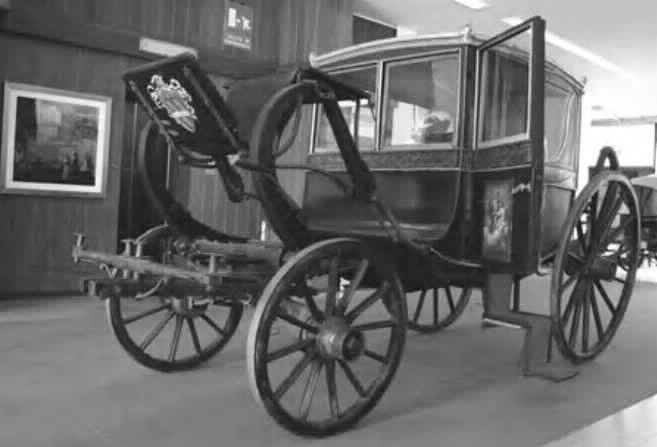
\includegraphics[width=0.4\textwidth]{2.1.png}
	\caption{This coach, built around 1650, shows a suspension made by four leaf springs and leader belts (National Automobile Museum of Torino). \cite{genta2014motorcar}
	}
	\label{fig:coach}
\end{figure}


\subsection{Suspension system evolution}
\begin{enumerate}
	\item \textbf{Passive Suspension Systems (Before 1980s):}
	\begin{itemize}
		\item Early automotive suspension systems were mostly passive, relying on mechanical components such as springs and dampers to absorb shocks and vibrations.
		\item These systems were simple and cost-effective but offered limited adaptability to varying road conditions.
	\end{itemize}
	\item \textbf{Active Suspension Systems (1980s - 1990s):}
	\begin{itemize}
		
		\item The concept of active suspension, which actively adjusts the suspension settings in response to changing road conditions, gained popularity in the 1980s.
		\item One of the pioneering examples was the development of the Lotus Active Suspension in Formula 1 in the late 1980s.
		\item Some high-end road cars began to incorporate active suspension systems in the late 1980s and early 1990s, including models from manufacturers like Citroën and Cadillac.
		\item Active suspension systems used sensors to monitor various factors, and electronic control systems adjusted the suspension settings in real-time to optimize ride comfort and handling.
	\end{itemize}
	
	\item \textbf{Semi-Active Suspension Systems (1990s - Present):}
	\begin{itemize}
		
		\item Semi-active suspension systems represent a middle ground between passive and active systems.
		\item In a semi-active system, the suspension settings are adjusted in real-time, but they typically do not provide as much active control as fully active systems.
		\item Popular semi-active systems include electronically controlled shock absorbers (e.g., Delphi's MagneRide) that can adjust damping rates based on driving conditions.
		\item These systems offer improved ride quality and handling without the complexity and cost associated with fully active systems.
	\end{itemize}
	
	\item \textbf{Recent Developments (2000s - Present):}
	\begin{itemize}
		
		\item Advancements in sensor technology, computing power, and materials have allowed for more sophisticated suspension systems.
		\item Active and semi-active suspension systems continue to evolve, with a focus on enhancing performance, safety, and comfort.
		\item Some modern high-performance and luxury vehicles feature advanced adaptive suspension systems that can adjust multiple parameters, including ride height, stiffness, and damping rates.
	\end{itemize}
\end{enumerate}
The semi-, figure \ref{fig:semi and active} (a), and fully-, figure \ref{fig:semi and active} (b), active suspension system are introduced. \cite{alashtari2023fuzzy}

\begin{figure}[H]
	\centering
	\begin{subfigure}{.35\textwidth}
		\centering
		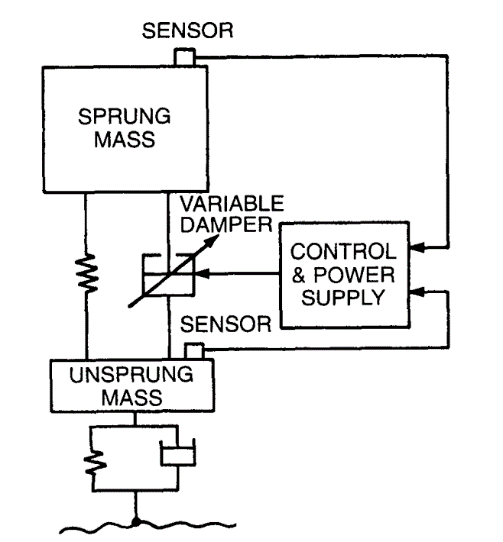
\includegraphics[width=\textwidth]{semi.png}
		\subcaption*{(a)}
	\end{subfigure}%
	\begin{subfigure}{.35\textwidth}
		\centering
		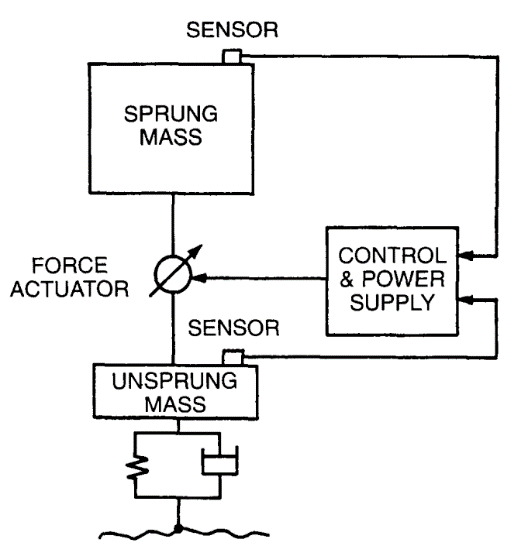
\includegraphics[width=\textwidth]{active.png}
		\subcaption*{(b)}
	\end{subfigure}
	\caption{Schematics of (a) Semi-active and (b) Fully-active suspension systems \cite{wong2001theory}}
	\label{fig:semi and active}
\end{figure}

Active suspension system is even beneficial for the HVG (Heavy Goods Vehicle) in case of the vehicle negotiating a turn.

\begin{figure}[H]
	\centering
	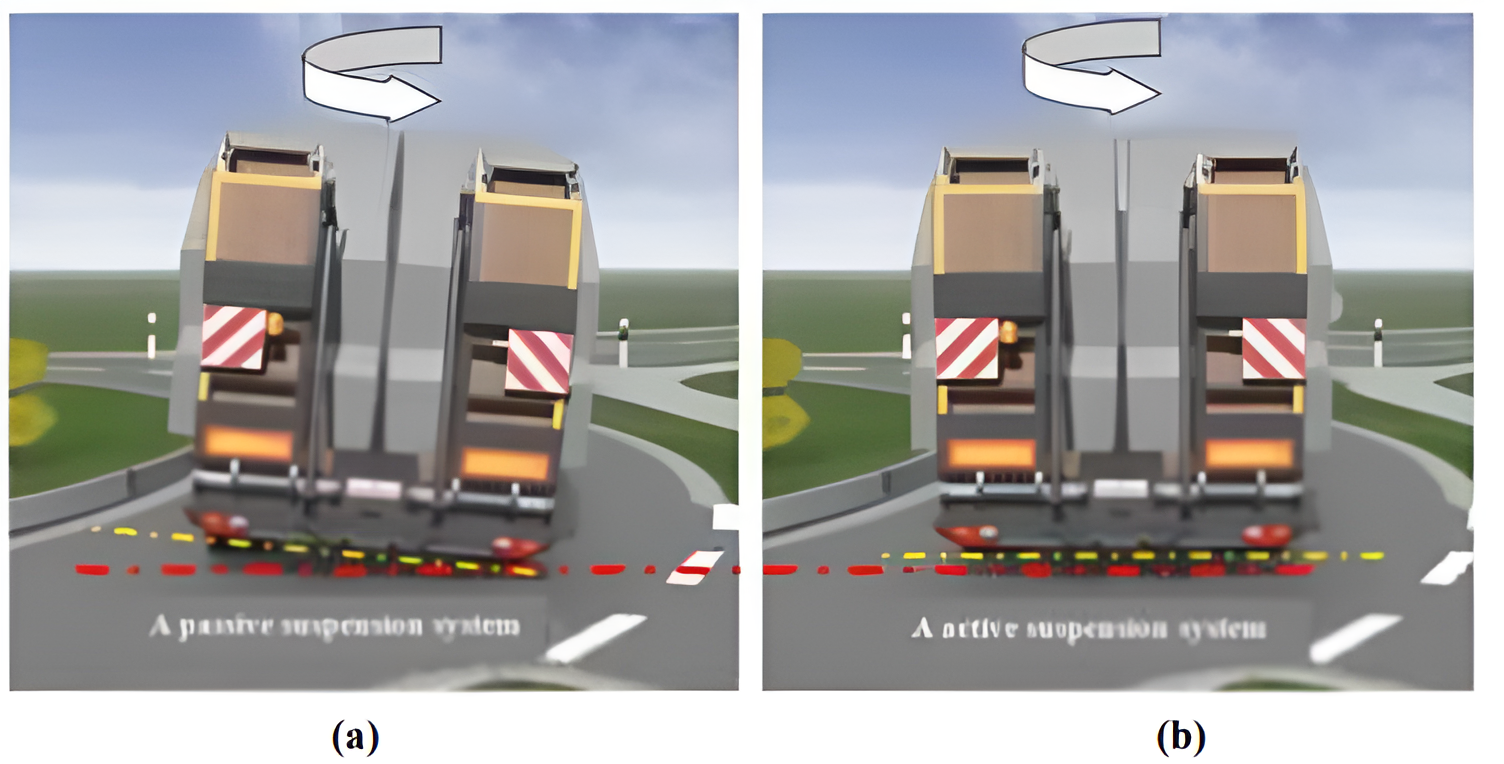
\includegraphics[width=.4\linewidth]{rolldef.png}
	\caption{Difference between the behavior of the truck body in a curve: with passive suspension (a) and with active suspension (b). \cite{hamza2022intelligent}}
	\label{fig:rolldef}
\end{figure}

\section{Recent Research}
\subsection{PID controller}
	Many studies on control problems for active suspension systems have been introduced in the last few decades. \cite{duong2022modeling} used PID (Proportional - Integral - Derivative) algorithm to control this system. This controller includes three stages corresponding to three coefficients, $K_p$, $K_D$ and $K_i$. These coefficients will be self-tuning or selected based on Ziegler-Nichols's method \cite{huba2021making}.

	However, the effectiveness of these methods is often low. \cite{chen2018modelling} used the Fuzzy algorithm to tune the PID controller's variables based on excitation signals from the road. Based on the principle of genetics, the variables of the PID controller can be optimally chosen by the GA (Genetic Algorithm) solution. This was done by \cite{metered2018optimized}.
	The size of the population and the number of generations will be determined based on the experience of the designer. Different from the GA algorithm, the PSO (Particle Swarm Optimization) method helps optimize the controller's coefficients based on the characteristics of the animals \cite{al2015quarter}. The animals used in this algorithm often have a herd lifestyle, such as whales, ants, bees, etc.  Besides, many other intelligent algorithms have been used to search for the controller's parameters optimally \cite{dahunsi2020proportional+}. 

	If the system has many objects to be controlled, PID can not be used, buy multiple PID controllers is an option\cite{nguyen2021improving}. 
	
\subsection{LQR controller}
	The Linear - Quadratic Regulator (LQR) controller can be used to replace the conventional PID controller for MIMO (Multi Input - Multi Output) systems\cite{wu2021multi}. This algorithm aims to minimize the cost function so the system can be more stable \cite{rodriguez2021active}. The mathematical model of this algorithm must be given in the form of a state matrix \cite{nguyen2022application}. Once the Gaussian filter is combined with the LQR controller, it will be called an LQG (Linear - Quadratic Gaussian) controller \cite{xia2015linear}.\newline
	
	Recent advancements in Linear Quadratic Regulator (LQR) control have led to significant developments in control theory and applications. For example, the LQR problem for singular systems has been revisited, focusing on enabling singular techniques for traditional control \cite{lqr_singular_systems}.
	
	Additionally, the role of predictions in online LQR control under stochastic and adversarial disturbances is examined \cite{lqr_predictions}, while data-driven LQR frameworks with stability guarantees are proposed using recursive learning and policy gradient methods \cite{lqr_stability_recursive}. 
	
\textbf{The above methods are only used for linear objects. If the object is nonlinear, more complex algorithms need to be used such as SMC MPC and RL.}




\subsection{SMC controller}
	The SMC algorithm is often used for complex nonlinear objects \cite{meetei2021enhanced}. Kazemian et al. used the SMC algorithm to control the hydraulic actuator. To simplify the model, a linearization process of a hydraulic actuator should be done. This process is shown by Nguyen \cite{nguyen2021advance}. Then, a quarter-dynamic model that considers the influence of the actuator will have five state variables \cite{nguyen2022novel}. According to Zhao et al. \cite{zhao2023sliding}, the sliding surface is an important component of the SMC controller. The controlled object can travel around the sliding surface in order to reach a steady state.
	
	The "chattering" is a phenomenon that can occur when this algorithm is used. This problem can make the control signal vibrate continuously with high frequency and a small amplitude. To limit this problem, an SMC controller must be combined with a PID controller or a Fuzzy controller. For instance, Hsiao and Wang \cite{hsiao2022evaluation} introduced the design of an algorithm that combines SMC and Fuzzy, called STFSMC (Self-tuning Fuzzy Sliding Mode Controller). Another recommendation has been made by Suhail et al. \cite{suhail2022adaptive} about using the ASMC (Adaptive Sliding Mode Control) algorithm. Overall, ride comfort can be greatly improved if this method is used \cite{wang2018nonlinear}. Besides, many advanced control methods have been applied to the active suspension system, which also brings high efficiency.

	
\subsection{RL controller}
	Recent advancements in the use of reinforcement learning for active suspension systems have shown promising results. For instance, a study on deep reinforcement learning for active suspension control highlights its potential for meeting ISO 2631-5 comfort requirements \cite{deep_rl_suspension}. Another research work introduced a TD3-based control algorithm to address actuator delays in active suspension systems \cite{td3_active_suspension}. 
	
	Optimization of full vehicle active suspension using advanced reinforcement learning controllers has also been explored, showcasing significant improvements in ride comfort \cite{ai_rl_full_vehicle}. Similarly, reinforcement learning-based vibration control for half-car active suspension systems demonstrated the effectiveness of adaptive dynamic programming algorithms \cite{rl_half_car}.
	
	The sim-to-real transfer of active suspension control has been studied to bridge the gap between simulated environments and real-world applications \cite{sim_to_real_rl}. Additionally, a novel approach using a closed-chain five-bar active suspension system with deep reinforcement learning provided promising results in stability and obstacle traversal \cite{closed_chain_rl}.
	
	Research into magnetorheological-damped vehicle suspension systems using RL showed that the TD3 algorithm outperforms traditional control strategies \cite{mr_damped_rl}. Finally, iterative learning-based reinforcement methods for road profile estimation and active suspension control in connected vehicles highlight the potential for collaborative frameworks \cite{iterative_learning_rl}.
	


	